\documentclass[border=3mm, tikz]{standalone}
\usepackage{graphicx,tikz} % Required for inserting images
\usetikzlibrary{calc}
\usepackage{xcolor}
\definecolor{crimson}{RGB}{ 170, 4, 36 }
\definecolor{darkblue}{RGB}{ 4, 47, 170 }
\begin{document}

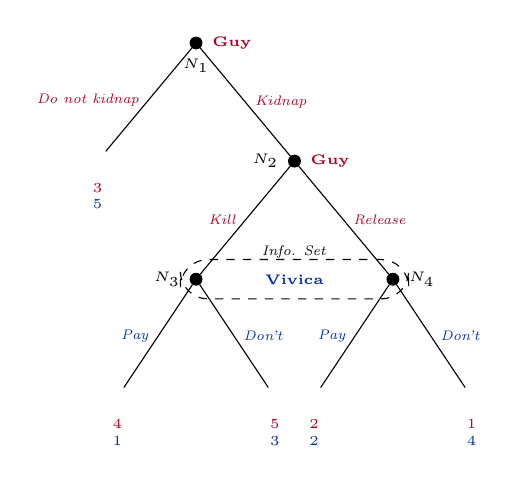
\begin{tikzpicture}[scale=1.0,font=\tiny]
\tikzstyle{solid node}=[circle,draw,inner sep=1.5,fill=black]
\tikzstyle{level 1}=[level distance=15mm,sibling distance=2.5cm]
\tikzstyle{level 2}=[level distance=15mm,sibling distance=2.5cm]
\tikzstyle{level 3}=[level distance=15mm,sibling distance=2cm]

\node(0)[solid node,label=right:{\textbf{\color{crimson} Guy}}, label=below:{$N_1$}]{}
    child{node[label=below:{
            \begin{tabular}{c}
                 {\color{crimson}  3} \\
                 {\color{darkblue} 5} \\
            \end{tabular}
        }
        ]{} 
    edge from parent node[left]{\textit{\color{crimson} Do not kidnap}}
    }
    child{node[solid node,label=right:{\textbf{\color{crimson} Guy}},
                          label=left:{$N_2$}]{} 
        child{node(1)[solid node, label=left:{$N_3$}]{} 
            child{node[label=below:{ 
                \begin{tabular}{c}
                     {\color{crimson}  4} \\
                     {\color{darkblue} 1} \\
                \end{tabular}
                }]{} 
            edge from parent node[left]{\textit{\color{darkblue} Pay}} 
            }
            child{node[label=below:{ 
                \begin{tabular}{c}
                     {\color{crimson}  5} \\
                     {\color{darkblue} 3} \\
                \end{tabular}
                }]{} 
            edge from parent node[right]{\textit{\color{darkblue} Don't}} 
            }
        edge from parent node[left]{\textit{\color{crimson} Kill}} 
        }
        child{node(2)[solid node, label=right:{$N_4$}]{} 
            child{node[label=below:{
                \begin{tabular}{c}
                    {\color{crimson}  2} \\
                    {\color{darkblue} 2} \\
                \end{tabular}
                }]{} 
            edge from parent node[left]{\textit{\color{darkblue} Pay}} 
            }
            child{node[label=below:{
                \begin{tabular}{c}
                     {\color{crimson}  1} \\
                     {\color{darkblue} 4} \\
                \end{tabular}
            }]{} 
            edge from parent node[right]{\textit{\color{darkblue} Don't}} 
            }
        edge from parent node[right]{\textit{\color{crimson} Release}} 
        }
    edge from parent node[right]{\textit{\color{crimson} Kidnap}}
    };

% information set
\draw[dashed,rounded corners=10]($(1) + (-.2,.25)$)rectangle($(2) +(.2,-.25)$);
% specify mover at 2nd information set
\node at ($(1)!.5!(2)$) {\textbf{\color{darkblue} Vivica}};
% label info set
\node at ($(1)!.5!(2) + (0,.35)$) {\textit{Info. Set}};


\end{tikzpicture}
\end{document}
